\begin{usecase}{Manage Scheduling Conflicts}
  \ucbasicinfo{Medium}{Regular}
  \ucshortdescription{This UC allows the user to manage scheduling conflicts by suggesting resolutions when overlapping events are detected.}
  \uctrigger{This UC is triggered when an automatically added event overlaps with an existing event.}
  \ucactors{User}{None}
  \ucpreconditions{
    \begin{itemize}
      \item User is logged in.
      \item Conflicting events list is not empty.
    \end{itemize}
  }
  \ucrelationships{N/A}{N/A}{N/A}
  \ucinputsoutputs{
    \begin{itemize}
      \item \textbf{Conflicting events} (Source: System)
      \item \textbf{Event to override} (Source: User)
    \end{itemize}
  }{
    \begin{itemize}
      \item \textbf{Conflict resolution suggestion} (Destination: User Interface)
      \item \textbf{Updated event schedules} (Destination: Calendar)
    \end{itemize}
  }
  \ucmainflow{
    \begin{enumerate}
      \item The user opens the application and clicks on the view conflicts icon
        \ucinfo{The application shows all the conflics with their resolution options}
      \item The user chooses the best fit option to manage each conflict 
        \ucinfo{The conflict is resolved and is removed from the conflict list }

    \end{enumerate}
  }
  \ucalternateflows{
    \begin{enumerate}
      \item If the user doesn't choose any option, it shows conflicting status until the user chooses any option or the event expires. 
      \item If the user clicks on reject the event is left overlapping.
    \end{enumerate}
  }
  \ucexceptions{
    \begin{itemize}
      \item Netwok failure 
    \end{itemize}
  }
  \ucconclusion{The UC ends when the conflicting events are either resolved or marked as conflicting, based on the user's choice.}
  \ucpostconditions{The calendar reflects the user's decision regarding event conflicts.}
  \ucspecialrequirements{The system should provide best suggestions for resolving conflicts.}
\end{usecase}

\begin{figure}[!h]
  \centering
  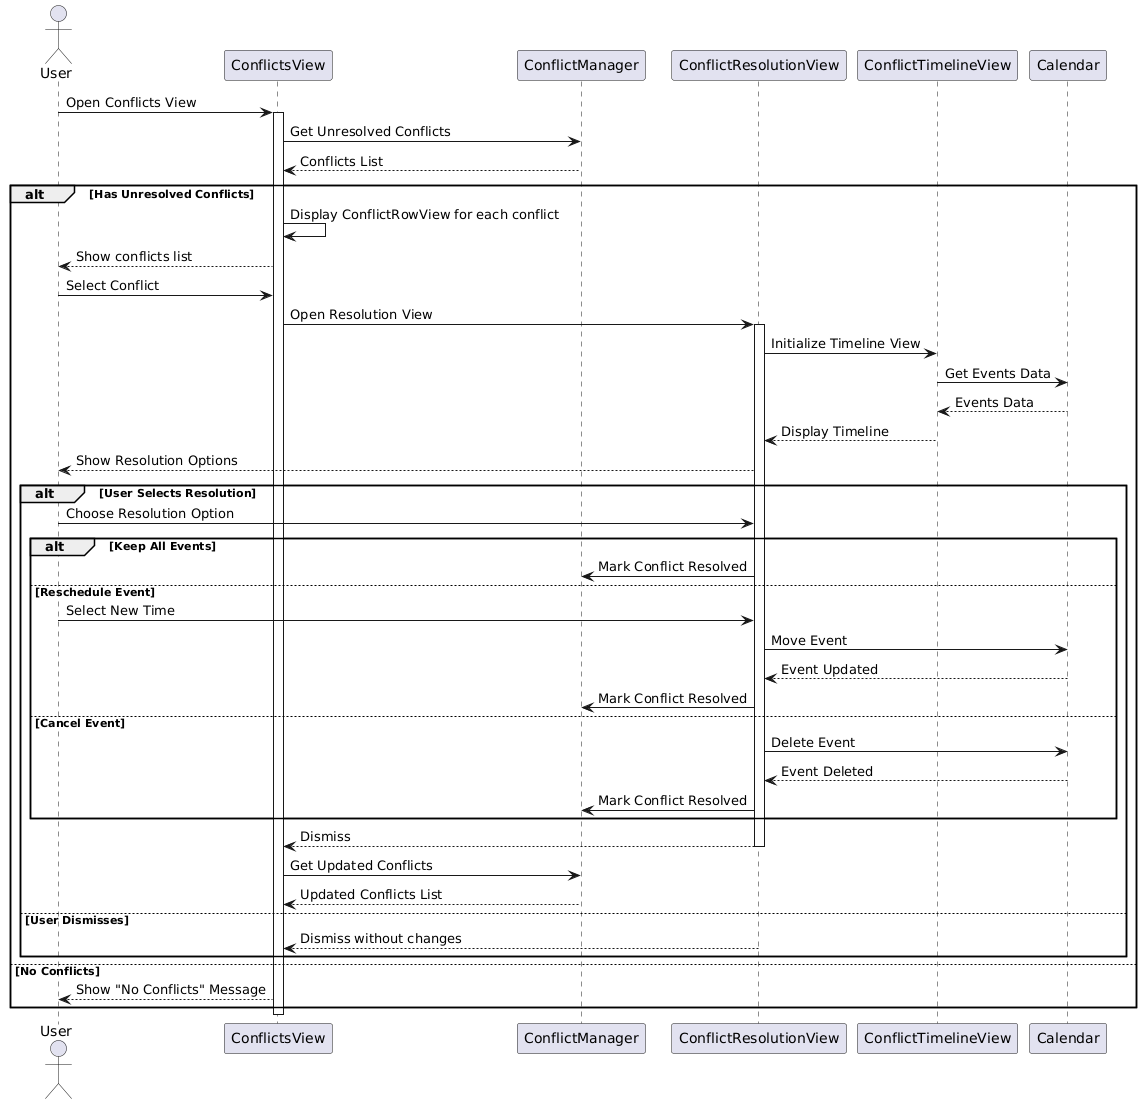
\includegraphics[width=\textwidth]{images/docs/diagrams/sequence-diagrams/all-sequence-diagrams/Manage Scheduling Conflicts.png}
  \caption{Manage Scheduling Conflicts Sequence Diagram}
  \label{fig:seq/manage-scheduling-conflicts}
\end{figure}